% THIS IS SIGPROC-SP.TEX - VERSION 3.1
% WORKS WITH V3.2SP OF ACM_PROC_ARTICLE-SP.CLS
% APRIL 2009
%
% It is an example file showing how to use the 'acm_proc_article-sp.cls' V3.2SP
% LaTeX2e document class file for Conference Proceedings submissions.
% ----------------------------------------------------------------------------------------------------------------
% This .tex file (and associated .cls V3.2SP) *DOES NOT* produce:
%       1) The Permission Statement
%       2) The Conference (location) Info information
%       3) The Copyright Line with ACM data
%       4) Page numbering
% ---------------------------------------------------------------------------------------------------------------
% It is an example which *does* use the .bib file (from which the .bbl file
% is produced).
% REMEMBER HOWEVER: After having produced the .bbl file,
% and prior to final submission,
% you need to 'insert'  your .bbl file into your source .tex file so as to provide
% ONE 'self-contained' source file.
%
% Questions regarding SIGS should be sent to
% Adrienne Griscti ---> griscti@acm.org
%
% Questions/suggestions regarding the guidelines, .tex and .cls files, etc. to
% Gerald Murray ---> murray@hq.acm.org
%
% For tracking purposes - this is V3.1SP - APRIL 2009

\documentclass{acm_proc_article-sp}

\begin{document}

%\title{A Sample {\ttlit ACM} SIG Proceedings Paper in LaTeX
%Format\titlenote{(Does NOT produce the permission block, copyright information nor page numbering). For use with ACM\_PROC\_ARTICLE-SP.CLS. Supported by ACM.}}
\title{ Classification of Crowdsourced Text Correction}

%\subtitle{[Extended Abstract]
%\titlenote{A full version of this paper is available as
%\textit{Author's Guide to Preparing ACM SIG Proceedings Using
%\LaTeX$2_\epsilon$\ and BibTeX} at
%\texttt{www.acm.org/eaddress.htm}}}
%
% You need the command \numberofauthors to handle the 'placement
% and alignment' of the authors beneath the title.
%
% For aesthetic reasons, we recommend 'three authors at a time'
% i.e. three 'name/affiliation blocks' be placed beneath the title.
%
% NOTE: You are NOT restricted in how many 'rows' of
% "name/affiliations" may appear. We just ask that you restrict
% the number of 'columns' to three.
%
% Because of the available 'opening page real-estate'
% we ask you to refrain from putting more than six authors
% (two rows with three columns) beneath the article title.
% More than six makes the first-page appear very cluttered indeed.
%
% Use the \alignauthor commands to handle the names
% and affiliations for an 'aesthetic maximum' of six authors.
% Add names, affiliations, addresses for
% the seventh etc. author(s) as the argument for the
% \additionalauthors command.
% These 'additional authors' will be output/set for you
% without further effort on your part as the last section in
% the body of your article BEFORE References or any Appendices.

\numberofauthors{3} %  in this sample file, there are a *total*
% of EIGHT authors. SIX appear on the 'first-page' (for formatting
% reasons) and the remaining two appear in the \additionalauthors section.
%
\author{
% You can go ahead and credit any number of authors here,
% e.g. one 'row of three' or two rows (consisting of one row of three
% and a second row of one, two or three).
%
% The command \alignauthor (no curly braces needed) should
% precede each author name, affiliation/snail-mail address and
% e-mail address. Additionally, tag each line of
% affiliation/address with \affaddr, and tag the
% e-mail address with \email.
%
% 1st. author
\alignauthor
Megha Gupta\\
       \affaddr{Dept. of Computer Science}\\
       \affaddr{IIIT-Delhi, India.}\\
       \email{meghag@iiitd.ac.in}
% 2nd. author
\alignauthor
Haimonti Dutta\titlenote{The author is also affiliated to the Institute of Data Science and Engineering (IDSE), Columbia University and is an adjunct professor at IIIT-Delhi.}\\
       \affaddr{Department of Management Science and Systems}\\
       \affaddr{State University of New York, Buffalo}\\
       \affaddr{New York, 14260}\\
       \email{haimonti@buffalo.edu}
% 3rd. author
\alignauthor 
Brian Geiger\\
       \affaddr{Center for Bibliographical Studies\\
and Research}\\
       \affaddr{University of California, Riverside.}\\
       \email{brian.geiger@ucr.edu}
       }
% There's nothing stopping you putting the seventh, eighth, etc.
% author on the opening page (as the 'third row') but we ask,
% for aesthetic reasons that you place these 'additional authors'
% in the \additional authors block, viz.
%\additionalauthors{Additional authors: John Smith (The Th{\o}rv{\"a}ld Group,
%email: {\texttt{jsmith@affiliation.org}}) and Julius P.~Kumquat
%(The Kumquat Consortium, email: {\texttt{jpkumquat@consortium.net}}).}
%\date{30 July 1999}
% Just remember to make sure that the TOTAL number of authors
% is the number that will appear on the first page PLUS the
% number that will appear in the \additionalauthors section.

\maketitle
\begin{abstract}
Optical Character Recognition (OCR) is a commonly used technique for digitizing printed material enabling them to be displayed online, searched and used in text mining applications. 
The text generated from OCR devices is often garbled due to variations in quality of the input paper, size and style of the font and column layout. This adversely affects retrieval effectiveness and hence techniques for cleaning the garbled text need to be improvised.%Often such techniques involve laborious and time consuming manual processing of data. This paper presents a prototype system for \textbf{C}lassification of \textbf{C}rowdsourced \textbf{T}ext \textbf{C}orrection (CCTC) which takes as input log files containing garbled and manually corrected OCR text, parses and tokenizes them and builds models for categorizing the corrections using state-of-the-art machine learning algorithms. Retrieval effectiveness on the California Digital Newspaper Collection is measured using mean reciprocal rank. 
This prototype system is expected to be deployed on historical newspaper archives that make extensive use of user text corrections.
\end{abstract}

% A category with the (minimum) three required fields
%\category{H.4}{Information Systems Applications}{Miscellaneous}
%A category including the fourth, optional field follows...
%\category{D.2.8}{Software Engineering}{Metrics}[complexity measures, performance measures]
%
%\terms{Theory}
%
%\keywords{ACM proceedings, \LaTeX, text tagging} % NOT required for Proceedings

\section{Introduction}
\label{sec:intro}
%Crowdsourcing is used extensively in cultural heritage and digital history related projects in recent years to digitize, create and process content and provide editorial or processing interventions. For example, the Australian Newspapers Digitization Program \cite{ADNP} allows communities to explore their rich newspaper heritage by enabling free online public access to over 830,000 newspaper pages containing 8.4 million articles. The public enhanced the data by correcting over 7 million lines of text and adding 200,000 tags and 4600 comments \cite{holley_09}. 
%%Picture Australia \cite{pictAus} harvests digital images from other heritage institutions and encourages the public to upload their own images and tag them. 
%FamilySearch \cite{famSearch} made available handwritten digital images of births, deaths and marriage records for transcription by the public. The New York Public Library has 1,277,616 dishes transcribed to date from 17,079 menus. 
%%Galaxy Zoo \cite{galZoo} is an online collaborative astronomy project in which users are invited to classify millions of galaxies from digital photos. 
%
%In all of the above crowdsourcing projects, large volumes of data are generated by users. These include tags, folksonomies, flagged content, information on history, relationship and preference data, structured labels describing objects and creative responses \cite{Ridge_11}. However, little statistical analysis is done of the user generated content in most cases. Assessment of data quality obtained by leveraging the ``wisdom of the crowd" remains an open problem. 
%
%%Before this question can be answered, statistical analysis of the data generated is imperative.

In this paper, we focus on understanding the nature of text corrections done by users of an old historic newspaper archive. 
%The newspapers are made available for searching on the Internet after the following processes take place: (1) the microfilm copy or paper original is scanned; %(2) master and Web image files are generated; 
%(2) metadata is assigned for each page to improve the search capability of the newspaper; (3) OCR software is run over high resolution images to create searchable full text.
% and (5) OCR text, images, and metadata are imported into a digital library software program. 
The OCR scanning process is far from perfect and the documents generated from it contains a large amount of garbled text. A user is presented with a high resolution image of a newspaper page along with erroneous or distorted text from the OCR and is expected to rectify the garbled words as appropriate. A prototype for a system that can be used for \textbf{C}lassification of \textbf{C}rowdsourced \textbf{T}ext \textbf{C}orrection (CCTC) is presented which can answer simple questions such as ``What are the different kinds corrections proposed by users?" and provide statistics generated from the correction process. The output from the system can be used to enhance search and retrieval.

The study used log files generated from text correction software in use at the California Digital Newspaper Collection (CDNC)%\footnote{http://cdnc.ucr.edu/cgi-bin/cdnc}, which contains over 400,000 pages of newspapers published in California between 1846-1922. 
%To date, the archive has approximately 1680 registered users who have corrected close to 2 million lines of text. 
%The corrections are primarily categorized as changes in spellings, punctuation rectification, addition of content or capitalization. A semi-automatic engine for classifying corrections based on support vector machines is designed.  
To the best of our knowledge, this is the first attempt to statistically analyze and model OCR error corrections provided by the crowd. We posit that such a classification system will be beneficial when attempting to compensate the annotators; it can also be used for task allocation if some users are more comfortable with certain type of corrections than others.

%In a bid to serve its patrons better, the CDNC crowdsourced the cleaning of OCR text. To date..
%\begin{figure*}[t]
%\centering
%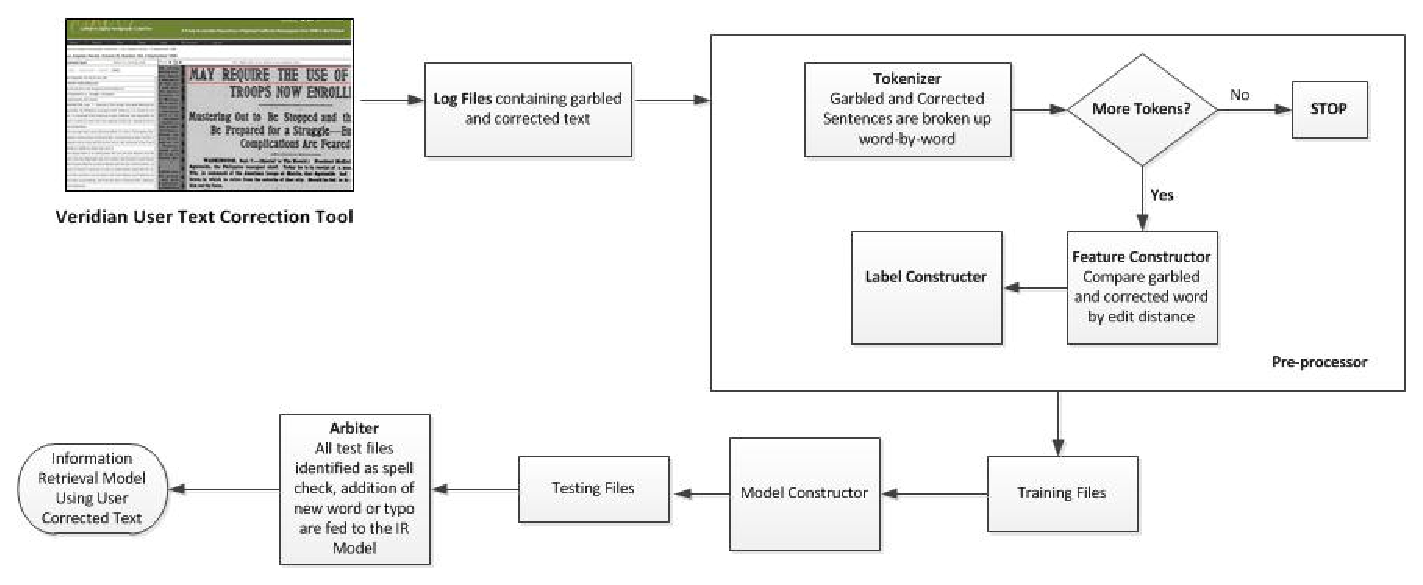
\epsfig{file=archOCR.eps, height= 3 in,width= 7 in}
%\caption{The Architecture of the Proposed System}
%\label{fig:arch}
%\end{figure*}

%\noindent \textbf{Organization}: Section~\ref{arch} describes the architecture of the proposed system; Section~\ref{sec:evaluation} presents empirical and scalability results on real-world data collected at CDNC; Section~\ref{ir} presents information retrieval techniques; Section~\ref{sec:related} discusses related work. Finally, Section~\ref{sec:conc} concludes the paper.
%




\section{System Components}
\label{components}
The \textbf{C}lassification of \textbf{C}rowdsourced \textbf{T}ext \textbf{C}orrection (CCTC) system has the following components:
\begin{enumerate}
\item The \textbf{Veridian User Text Correction}%\footnote{http://veridiansoftware.com/crowdsourcing/} tool which takes as input a scanned page of the newspaper and enables users to correct OCR errors as they come across them.
\item \textbf{Log Files: }All corrections performed by the annotators are recorded in log files.
%To date approximately 1,705,149 lines have been edited by 848 annotators which resulted in 235 log files. A sample of 191 files has been used for this work. Each log file is generated at the issue-level and contains XML data about the pages in the issue.
The following information is provided about the corrections:
%\begin{enumerate}
(a) \textit{Page Id: } The id of the page in which editing was done.
(b) \textit{Block Id: } The id of the paragraph containing the line corrected by the user.
(c) \textit{Line Id }
(d) \textit{Old Text Value} is the garbled text generated by the OCR device and replaced by the user.
(e) \textit{New Text Value} is the corrected text with which the old text was replaced.
%\end{enumerate}

\item \textbf{Preprocessor: } The preprocessor has three main components:
\begin{itemize}
\item \textbf{Tokenizer: } The old text and the new text from the log file is tokenized by white-spaces resulting in total 44,022 tokens of which 21,108 are corrected by the annotators.
\item \textbf{Feature Constructor: }\\
\textbf{Word-level feature construction:}
%Features are crafted by computing the Levenshtein edit distance between the old word and its correction. Six binary features are generated as follows: 
(a) \textbf{Difference Length Zero} : $1$, if both the old word and new word have same length and $0$ otherwise. 
%For example, the feature is 1 for the tokens ``Spll," and ``Union" as  both the tokens have same number of characters.
(b) \textbf{Difference Length Above One} : $1$, if the length of new word exceeds the length of old word and $0$ otherwise.
(c) \textbf{Edit Distance One}:  $1$, if single edit operation is required to convert old word to new word and $0$ otherwise. %For example, the feature is 1 for tokens ``Under" and ``under" or ``the" and ``them".
(d) \textbf{Edit Distance Above One}: $1$, if more than one edit operation is required to convert old word to new word and $0$ otherwise. %For ``Spll," and ``Union", value is 1 as more than one edit operation is required to convert from old to new token.
%(d) \textbf{Edit Distance Below Three}: 1, if less than three edit operations are required to convert old word to new word and $0$ otherwise. 
%For ``Stales" and ``Stables", value is 1 as less than three edit operations are required to convert from old to new token. 
(e) \textbf{Edit Distance is 1 and Case Change}: 1, if the two words have edit distance is exactly 1 and the first character of one string change from upper case to lower case or vice versa. %For example, for ``Stales" and ``Stables", the value is 0 as there is no case change.
(f) \textbf{Punctuation Difference}: 1, if both the old text and new text differ in any of the following punctuation marks (!"\#\$\%\&'*+,-./:;\textless=\textgreater?@[$\backslash$]\^\_`\{\textbar\}\textasciitilde).

\textbf{Character-level feature construction:}
The tokenization process of the text in the log files was modified to enable the addition and deletion classification of text using a character. 
%If the text was deleted by the user as a part of correction process then the character ``$\sim$" was assigned to the new token denoting that the user performed the task of deleting the OCR garbled text whereas if the user added a new text  then the character ``+" was assigned to the old token denoting that user added text that was initially missing in the OCR data.\\
The corrected tokens were split into character-level data contributing $58,963$ instances. Of $58,963$ instances, we encountered that $55,612$ had same character-level corrections indicating that the OCR makes the same type of mistakes repeatedly. The maximum number of redundant corrections noted were deletion of punctuations and special characters. %There were $4344$ deletions of comma, $2831$ deletions of $\ddot{A}$. Amongst character to character corrections, $635$ cases of o$\rightarrow$e, $470$ cases of b$\rightarrow$h, 299 cases of u$\rightarrow$n contributed maximum to the redundancy. The first graph in figure ~\ref{fig:o_e}(See Appendix) shows that the total corrections from the original word ``tbe" to the corrected word ``the" are $269$. 
%The x-axis in the graph denotes the examples of character-level corrections whereas the y-axis denotes the number of corrections made on the examples in the entire corpus. 
In order to test the performance of the manually crafted (word-level) features of the dataset, we used association rule mining algorithm to generate rules. Hence, the character-level feature construction acts as a baseline method.
%Apriori algorithm \cite{Agrawal1994} implementation of WEKA 3.7.10 was used to mine character-level rules. Mining association rules is to discover all the strong rules in the database using different measures of interestingness. To select interesting rules from the total set of possible rules, we use some user controlled measures like minimum support ($minsup$) and minimum confidence ($minconf$). They are formally defined as follows. \\
%Support(X$\rightarrow$Y) = P(X $\cup$ Y)\\
%represents the percentage of transactions from the transaction database that contains both X and Y.\\
%Confidence(X$\rightarrow$Y) = P(Y|X)\\ 
%represents the probability that the transaction containing X also contains Y.
%In our case, the value of $minconf$ and the the lower bound $minsup$ was set to $0.0001$, and the upper bound of $minsup$ was set to $1$. The upper bound of $minsup$ was iteratively decreased by a factor of $delta$ until either the lower bound of $minsup$ was reached or the required number of rules were generated.\\
The number of features and instances are $6631$ and $3351$ respectively in the character-level data set.
%\begin{figure*}[t]
%\centering
%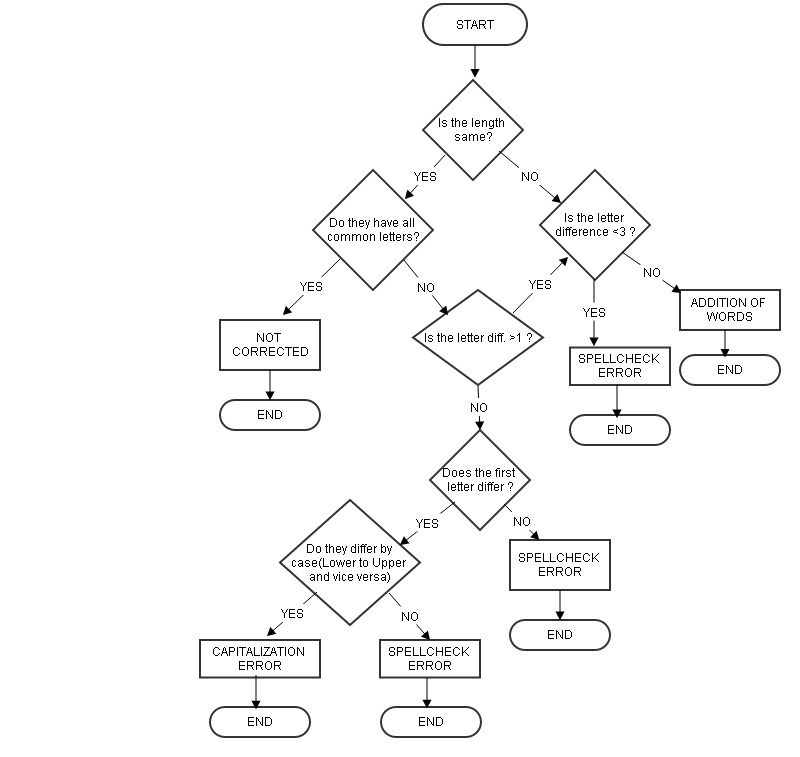
\includegraphics[width=0.9\textwidth]{./image/flowchartnew.jpg}
%%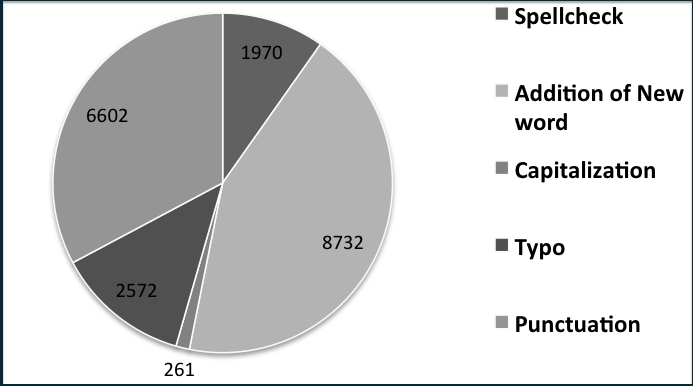
\includegraphics[width=6cm,height=4cm]{./image/error.jpg}
%\caption{Flowchart demonstrating how the labels are generated.}
%\label{fig:flowchart}
%\end{figure*}

%\begin{figure*}[ht]
%\centering
%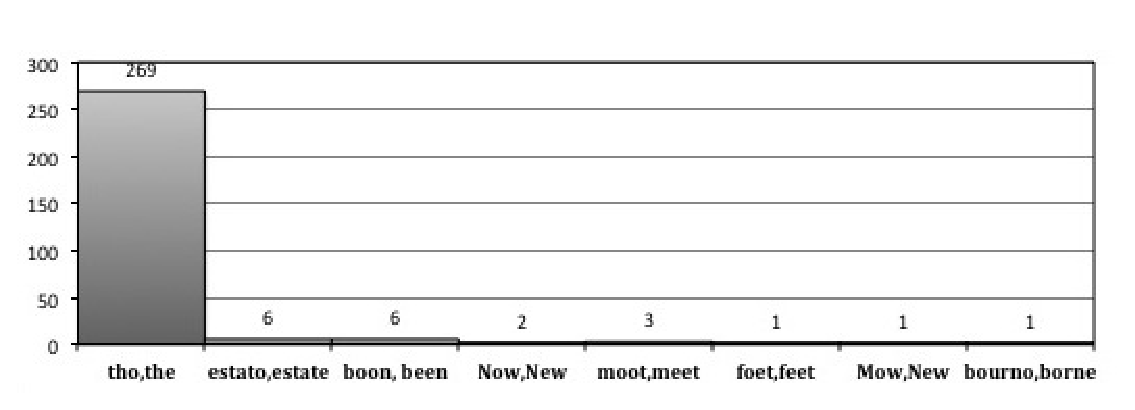
\epsfig{file=stat1edit.eps, height= 1.8 in,width= 3.4 in}
%\label{fig:stat1}
%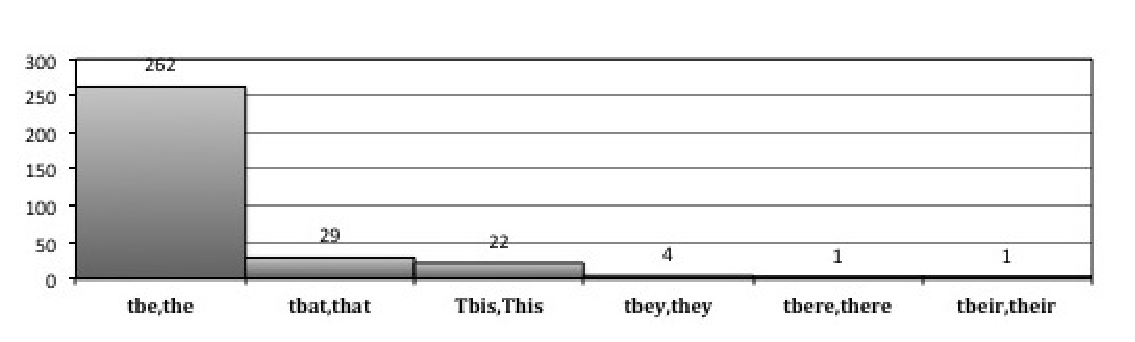
\epsfig{file=stat2copy.eps, height= 1.7 in,width= 3.3 in}
%\label{fig:stat2}
%%\epsfig{file=stat3copy.eps, height= 1.7 in,width= 3 in}
%%\label{fig:stat3}
%\caption{Examples of character level corrections}
%\end{figure*}

\item \textbf{Label Constructor: }
%The logic used in generation of the features can be summarized by the flowchart depicted in Figure~\ref{fig:flowchart}.
(a) \textbf{Addition: } When the length of new string exceeds the length of old given the difference is made by alphanumeric characters and the edit distance is above one. %For example, ``6RAVR" and ``GRAVEL".
(b) \textbf{Deletion: }When the length of old string exceeds the length of new given the difference is made by alphanumeric characters and the edit distance is above one. %For example, ``VVe" and ``We".
(c) \textbf{Punctuation: }When the difference in the length of strings is non-zero and they differ by special characters contained in the set (!"\#\$\%\&'()*+,-./:;\textless=\textgreater?@[$\backslash$]\^\_`\{\textbar\}\textasciitilde). %For example, ``Ladies!" and ``Ladies".
(d) \textbf{Capitalization: }When both the strings have equal length, edit distance is exactly 1 and first letter of both the strings change from upper to lower case or vice versa.% For example, ``largest" and ``Largest".
(e) \textbf{Spellcheck: }When the difference between string is above zero and the edit distance contributed by alphanumeric character is exactly one or when the strings have same length and the edit distance is one or above one irrespective of the involvement of special characters.% For example, ``the" and ``them" or ``hanger" and ``banger".

%The distribution of the these classes in the dataset is shown in Table~\ref{table: classes}.
It must be noted that by design tokens are always assigned to one class, although in principle it may be possible to assign them to multiple classes\footnote{For e.g. a correction of ``t$\$$e" to ``the" could be either a Spellcheck or a Punctuation Error correction but we assign it to Spellcheck }.
\end{itemize}


%\item \textbf{Model Construction: } The model for classifying crowdsourced text correction is built using a Multiclass Support Vector Machine algorithm \cite{Tsochantaridis_2004}. Each training point belongs to one of $k$ different classes. The goal is to construct a function, which given a new data point, will correctly predict the class to which it belongs.

\item \textbf{Model Construction: } The model for classifying crowdsourced text correction is built using a Multiclass Support Vector Machine algorithm\footnote{http://www.cs.cornell.edu/people/tj/svm\_light/svm\_multiclass.html}. Each training point belongs to one of $k$ different classes. The goal is to construct a function, which given a new data point, will correctly predict the class to which it belongs.

%Different methods have been proposed in literature for solving the SVM multi-class classification problem. Some popular techniques include: a) \textit{One-Versus-All (OVA) classification} Build $k$ different binary classifiers; for the $i^{th}$ classifier, let the positive examples be all points in class $i$ and negative examples not in class $i$. Let $f(x) = \text{arg } max_i f_i(x) $.  b) \textit{one-versus-one} uses the majority voting strategy where each classifier assigns the new instance one of two classes. The class with the majority votes is assigned to the instance.
%
%Crammer and Singer \cite{crammer} pose the multi-class classification problem as a single optimization problem, rather than decomposing it into multiple binary classification problems. A comparison of the above approaches can be found here \cite{comparison}.
%
%For a training set $(x_1,y_1) ... (x_n,y_n)$ with labels $y_i \in \{1, \cdots, k\}$, the multi class problem can be posed as a constrained optimization problem with a quadratic objective function:
%$\text{min } \frac{1}{2} \sum_{i = 1}^{k} \parallel w_{i}\parallel^2 + \frac{C}{n} \sum_{i = 1}^{n}\xi_{i} $
%
%s.t. $\forall y \leq k : [x_{1} \cdot w_{yi}] \geq [x_{1} \cdot w_{y}] + 100*\Delta(y_{1},y)-\xi_{1}$
%$\cdots$
%s.t. $\forall y \leq k : [x_{n} \cdot w_{yn}] \geq [x_{n} \cdot w_{y}] + 100*\Delta(y_{n},y)-\xi_{n}$
%
%Here $C$ is the regularization parameter, $\Delta(y_{j},y), 1 \le j \le n$ is the loss function that returns 0 if $y_{j}$ equals y, and 1 otherwise and $\xi_{i}, 1 \le i \le n$ are the non negative slack variables which measure the degree of misclassification of the instance $x_{i}$. 
%%\cite{algo} has to two modules, \textit{svm\_multiclass\_learn} and \textit{svm\_multiclass\_classify}. The learning module learns the model given the parameters and the training data whereas the classification module applies the learned model to the test data to find the error. 
%It must be noted that when the data is not linearly separable, the following kernel functions are used for classification:
%%the original finite dimensional space is mapped to a much higher dimensional space in order to make the separation easier in that space. The mappings used by SVM schemes are designed to ensure that the dot products may be computed easily in terms of the variables in the original space, by defining them in terms of a Kernel function selected to suit the problem. The types of kernel function used can be described as follows:\\
%a) Linear Kernel: $K(x,y) = x^{T}y + c $
%b) Polynomial Kernel : $K(x,y) = (\alpha x^{T}y + c)^{d}$
%c) Radial Basis Kernel : $K(x,y) = exp(-\lvert \lvert x-y\rvert\rvert^{2}/2\sigma^{2}$)


\item \textbf{Information Retrieval Techniques: }The main aim of this system is to improve the quality of text for use with an IR system. The metric used for evaluation here is mean reciprocal rank (MRR) which produces a list of possible ranked responses to a sample of queries, Q. The reciprocal rank is the multiplicative inverse of the rank of the first correct answer. The first correct answer is decided by the users. The average of the reciprocal ranks over a sample of queries is the mean reciprocal rank. The higher value of the MRR in the case of corrected corpus indicates that the relevant results are ranked higher in the retrieved set of documents.

\end{enumerate}

%This article shows only the plainest form
%of the citation command, using \texttt{{\char'134}cite}.
%This is what is stipulated in the SIGS style specifications.
%No other citation format is endorsed.
%

%To set a wider table, which takes up the whole width of
%the page's live area, use the environment
%\textbf{table*} to enclose the table's contents and
%the table caption.  As with a single-column table, this wide
%table will ``float" to a location deemed more desirable.
%Immediately following this sentence is the point at which
%Table 2 is included in the input file; again, it is
%instructive to compare the placement of the
%table here with the table in the printed dvi
%output of this document.
%
%
%As was the case with tables, you may want a figure
%that spans two columns.  To do this, and still to
%ensure proper ``floating'' placement of tables, use the environment
%\textbf{figure*} to enclose the figure and its caption.
%
%Note that either {\textbf{.ps}} or {\textbf{.eps}} formats are
%used; use
%the \texttt{{\char'134}epsfig} or \texttt{{\char'134}psfig}
%commands as appropriate for the different file types.
%
%
%\subsection*{A {\secit Caveat} for the \TeX\ Expert}
%Because you have just been given permission to
%use the \texttt{{\char'134}newdef} command to create a
%new form, you might think you can
%use \TeX's \texttt{{\char'134}def} to create a
%new command: \textit{Please refrain from doing this!}
%Remember that your \LaTeX\ source code is primarily intended
%to create camera-ready copy, but may be converted
%to other forms -- e.g. HTML. If you inadvertently omit
%some or all of the \texttt{{\char'134}def}s recompilation will
%be, to say the least, problematic.
\section{Results}
 The performance of the algorithm is evaluated using 10-fold cross validation technique. The \textbf{A}verage loss \textbf{E}rror (AE) and  \textbf{A}verage running \textbf{T}ime (AT) from cross validation for baseline (character-level) and proposed (word-level) dataset respectively are represented as $AE_{b}$, $AE_{p}$. Table ~\ref{table: errors} shows the result of the experiment, error and running time (cpu seconds) using linear kernel for different values of $C$. Table~\ref{table: kernels} shows the result of the experiment, error and running time (cpu minutes) using polynomial and radial basis kernel.\\
The multi-class SVM algorithm using polynomial kernel gives the best results in both the datasets, word-level and character-level. In case of automatically generated character-level dataset, the performance of the algorithm does not improve by varying the regularization constant in contrast to the performance of the manually crafted word-level dataset. In case of word-level dataset, as the value of regularization constant increases, the average loss of the learning model decreases. However, the time taken to train the model is considerably high. Thus, one can learn less accurate but faster models with linear or RBF kernels. Thus, it may be useful to consider a trade-off between accuracy of learnt models versus time taken for classification in large scale deployments.
\begin{table}[htdp]
\centering
\caption{Results using linear kernel}
\begin{tabular}{|lllll|}
\hline
C &$AE_{b}$&$AE_{p}$&$AT_{b}$&$AT_{p}$\\
\hline
.0001&99.43$\pm .09$&49.47$\pm0.25$&1.268$\pm.06$&0.11$\pm.01$\\
.1&99.43$\pm .09$&49.464$\pm .47$&2.512$\pm0.01$&0.061$\pm0.01$\\
10&99.43$\pm .09$&4.974$\pm .5$&2.512$\pm0.01$&0.17\\
1000&99.43$\pm .09$&1.743$\pm .14$&3.635$\pm0.08$&0.382$\pm0.04$\\
10000&99.43$\pm .09$&0&6.126$\pm0.02$&0.303$\pm0.02$\\
\hline
\end{tabular}
\label{table: errors}
\end{table}
\vspace{-2em}
\begin{table}[htdp]
\centering
\caption{Results using polynomial and rbf kernels}
\begin{tabular}{|l|ll|ll|}
\hline
&Polynomial&&RBF&\\
\cline{2-5}
C&$AE_{b}$ & $AE_{p}$&$AE_{b}$&$AE_{p}$\\
\hline
.0001&42$\pm.13$&50$\pm.47$&63$\pm.15$&27$\pm.5$\\
100&42$\pm.13$&.33$\pm.2$&63$\pm.16$&3$\pm.4$\\
1000&42$\pm.13$&0$\pm0$&63$\pm.16$&1.7$\pm.2$\\
\hline
C&$AT_{b}$ & $AT_{p}$ &$AT_{b}$ & $AT_{p}$ \\
 \hline
.0001&37$\pm1.4$&10$\pm0.2$&25$\pm0.7$&6$\pm0.2$\\
100&326$\pm11.8$&1239$\pm118$&$540\pm110$&404$\pm34$\\
1000&942$\pm17.4$&764$\pm93$&537$\pm111.72$&957$\pm184$\\
\hline
\end{tabular}
\label{table: kernels}
\end{table}


%\begin{table*}
%\parbox{.51\linewidth}{
%\centering
%\caption{Results using linear kernel}
%\begin{tabular}{|lllll|}
%\hline
%C &$AE_{b}$&$AE_{p}$&$AT_{b}$&$AT_{p}$\\
%\hline
%.0001&99.43$\pm .09$&49.47$\pm0.25$&1.268$\pm.06$&0.11$\pm.01$\\
%.1&99.43$\pm .09$&49.464$\pm .47$&2.512$\pm0.01$&0.061$\pm0.01$\\
%10&99.43$\pm .09$&4.974$\pm .5$&2.512$\pm0.01$&0.17\\
%1000&99.43$\pm .09$&1.743$\pm .14$&3.635$\pm0.08$&0.382$\pm0.04$\\
%10000&99.43$\pm .09$&0&6.126$\pm0.02$&0.303$\pm0.02$\\
%\hline
%\end{tabular}
%\label{table: error}
%}
%\hfill
%\parbox{.51\linewidth}{
%\centering
%\caption{Results using polynomial and rbf kernels}
%\begin{tabular}{|l|ll|ll|}
%\hline
%&Polynomial&&RBF&\\
%\cline{2-5}
%C&$AE_{b}$ & $AE_{p}$&$AE_{b}$&$AE_{p}$\\
%\hline
%.0001&42$\pm.13$&50$\pm.47$&63$\pm.15$&27$\pm.5$\\
%100&42$\pm.13$&.33$\pm.2$&63$\pm.16$&3$\pm.4$\\
%1000&42$\pm.13$&0$\pm0$&63$\pm.16$&1.7$\pm.2$\\
%\hline
%C&$AT_{b}$ & $AT_{p}$ &$AT_{b}$ & $AT_{p}$ \\
% \hline
%.0001&37$\pm1.4$&10$\pm0.2$&25$\pm0.7$&6$\pm0.2$\\
%100&326$\pm11.8$&1239$\pm118$&$540\pm110$&404$\pm34$\\
%1000&942$\pm17.4$&764$\pm93$&537$\pm111.72$&957$\pm184$\\
%\hline
%\end{tabular}
%\label{table: kernels}
%}
%\end{table*}


\section{Conclusions}
In this paper, we present a system for Classification of Crowdsourced Text Correction which is capable of modelling user corrections using state-of-the-art machine learning techniques and retrieve categories which are likely to enhance search on the archive such as addition of words, elimination of typographical errors or addition of content. We also compared the two datasets, word-level and character-level by applying the machine learning algorithms on each. The manually crafted word-level dataset performed better in terms of average loss error. However, the running time of the algorithm was considerably high. Thus, there is a need to improve the algorithms in order to make them compatible with large scale datasets.\\
%Information retrieval metric, mean reciprocal rank is used to quantify the effectiveness of the user text correction. The higher value of the MRR in the case of corrected corpus indicates that the relevant results are ranked higher in the retrieved set of documents.
%\end{document}  % This is where a 'short' article might terminate

%ACKNOWLEDGMENTS are optional
%\section{Acknowledgments}
%This section is optional; it is a location for you
%to acknowledge grants, funding, editing assistance and
%what have you.  In the present case, for example, the
%authors would like to thank Gerald Murray of ACM for
%his help in codifying this \textit{Author's Guide}
%and the \textbf{.cls} and \textbf{.tex} files that it describes.

%
% The following two commands are all you need in the
% initial runs of your .tex file to
% produce the bibliography for the citations in your paper.
%\bibliographystyle{abbrv}
%\bibliography{sigproc-sp}  % sigproc.bib is the name of the Bibliography in this case
% You must have a proper ".bib" file
%  and remember to run:
% latex bibtex latex latex
% to resolve all references
%
% ACM needs 'a single self-contained file'!

\balancecolumns
% That's all folks!
\end{document}
